% context: markscheme (official solutions) for 2-7CW_Graphing-free-fall
% topic: graphs of free fall with g rounded to 10 m/s^2; y vs t a half parabola,
%        v vs t a line of slope g; chord = average velocity, tangent = instantaneous
%        velocity; a ball thrown up at 15 m/s
% convention: answers in bold; "=" joins exact equalities, "\approx" introduces a
%        rounded value
\documentclass[12pt, twoside]{article}
%\documentclass[12pt, twoside]{article}
\usepackage[letterpaper, margin=1in, headsep=0.2in]{geometry}
\setlength{\headheight}{0.6in}
%\usepackage[english]{babel}
\usepackage[utf8]{inputenc}
\usepackage{microtype}
\usepackage{amsmath}
\usepackage{amssymb}
%\usepackage{amsfonts}
\usepackage[nomessages]{fp} %\FPeval{\var-name}{2*sin(pi/6)}
\usepackage{siunitx} %units in math. eg 20\milli\meter
\usepackage{yhmath} % for arcs, overparenth command
\usepackage{tikz} %graphics
\usetikzlibrary{quotes, angles, arrows, arrows.meta}
\usepackage{graphicx} %consider setting \graphicspath{{images/}}
\usepackage{parskip} %no paragraph indent
\usepackage{enumitem}
\usepackage{multicol}
\usepackage{venndiagram}

\usepackage{fancyhdr}
\pagestyle{fancy}
\fancyhf{}
\renewcommand{\headrulewidth}{0pt} % disable the underline of the header
\raggedbottom
\hfuzz=2mm %suppresses overfull box warnings

\usepackage{hyperref}
\usepackage{float}
\setlength{\parskip}{0.2\baselineskip}

\title{Physics}
\author{Chris Huson}
\date{November 2026}

\fancyhead[LE]{\thepage}
\fancyhead[RO]{\thepage}
\fancyhead[LO]{La Scuola d'Italia / Huson / Physics \\* 12 November 2026}

\begin{document}

\subsubsection*{2.7 Classwork: Graphing Free Fall Solutions}

\begin{enumerate}[itemsep=0.4cm]

\item $v = 10\,t$ gains 5 m/s every half second. For $y = 5\,t^2$, square the time
  first.

  {\renewcommand{\arraystretch}{1.4}%
  \begin{tabular}{| l | c | c | c | c | c | c | c |}
    \hline
    $t$ (s) & 0 & 0.5 & 1.0 & 1.5 & 2.0 & 2.5 & 3.0 \\ \hline
    $v$ (m/s) & \textbf{0} & \textbf{5} & \textbf{10} & \textbf{15} & \textbf{20} &
      \textbf{25} & \textbf{30} \\ \hline
    $y$ (m) & \textbf{0} & 1.25 & \textbf{5} & \textbf{11.25} & \textbf{20} &
      \textbf{31.25} & \textbf{45} \\ \hline
  \end{tabular}}

  \emph{For example $y(1.5) = 5 \times 1.5^2 = 5 \times 2.25 = 11.25$ m. The common
  slip is $1.5^2 = 2.5$ or $0.5^2 = 2.5$, the same error as $0.2^2 = 0.4$ on 2-6DN.
  With $g = 9.80$ m/s$^2$ the values are 2\% smaller (4.90 m at 1.0 s, 44.1 m at
  3.0 s), too little to see on these grids.}

\item \textbf{Graphs.} Below, with the chord and tangent of Question 3 drawn on the
  position graph.

  \begin{tikzpicture}[x=1.95cm, y=0.135cm]
    \draw[gray!25, thin, xstep=0.1, ystep=1] (0,0) grid (3,45);
    \draw[gray!60, xstep=0.5, ystep=5] (0,0) grid (3,45);
    \draw[->, thick] (0,0) -- (3.12,0) node[below right]{\small $t$ (s)};
    \draw[->, thick] (0,0) -- (0,47.5) node[above]{\small $y$ (m)};
    \foreach \t in {0,0.5,1.0,1.5,2.0,2.5,3.0} \node[below] at (\t,0) {\scriptsize \t};
    \foreach \y in {5,10,...,45} \node[left] at (0,\y) {\scriptsize \y};
    \node[above] at (1.5,47.5) {\small Position};
    \draw[very thick, domain=0:3, samples=60] plot (\x, {5*\x*\x});
    \foreach \t in {0,0.5,1,1.5,2,2.5,3} \fill (\t, {5*\t*\t}) circle (1.5pt);
    \draw[thick, dashed] (1,5) -- (2,20) node[pos=0.55, left]{\scriptsize (a)};
    \draw[thick, dotted] (0.5,0) -- (2.2,17) node[right]{\scriptsize tangent};
  \end{tikzpicture}
  \hfill
  \begin{tikzpicture}[x=1.95cm, y=0.2025cm]
    \draw[gray!25, thin, xstep=0.1, ystep=1] (0,0) grid (3,30);
    \draw[gray!60, xstep=0.5, ystep=5] (0,0) grid (3,30);
    \draw[->, thick] (0,0) -- (3.12,0) node[below right]{\small $t$ (s)};
    \draw[->, thick] (0,0) -- (0,31.7) node[above]{\small $v$ (m/s)};
    \foreach \t in {0,0.5,1.0,1.5,2.0,2.5,3.0} \node[below] at (\t,0) {\scriptsize \t};
    \foreach \v in {5,10,...,30} \node[left] at (0,\v) {\scriptsize \v};
    \node[above] at (1.5,31.7) {\small Velocity};
    \draw[very thick] (0,0) -- (3,30);
    \foreach \t in {0,0.5,1,1.5,2,2.5,3} \fill (\t, {10*\t}) circle (1.5pt);
  \end{tikzpicture}

  \begin{enumerate}[itemsep=0.25cm]
    \item \textbf{No, it curves upward} (half of a parabola). The slope of the
      position graph is the velocity, so a steeper and steeper curve means
      \textbf{the stone is going faster and faster}. It falls 1.25 m in the first
      half second but 13.75 m in the last.
    \item \textbf{At $\mathbf{t = 0}$ the stone is at rest}: it is dropped, so
      $v_0 = 0$, and a slope of zero means a velocity of zero.
    \item Using (0, 0) and (3.0 s, 30 m/s): slope $= \dfrac{30 - 0~\text{m/s}}{3.0 - 0~\text{s}}
      = \mathbf{10~\textbf{m/s}^2}$. \textbf{The slope is the acceleration, $\mathbf{g}$.}

      \emph{Units: m/s divided by s is m/s$^2$. Accept any two points on the line.}
  \end{enumerate}

\newpage

\item \textbf{Chords and a tangent.} Values are from the table; readings from a
  hand-drawn graph within about 1 m/s are fine.
  \begin{enumerate}[itemsep=0.3cm]
    \item slope $= \dfrac{\Delta y}{\Delta t} = \dfrac{20 - 5~\text{m}}{2.0 - 1.0~\text{s}}
      = \mathbf{15~\textbf{m/s}}$
    \item slope $= \dfrac{11.25 - 5~\text{m}}{1.5 - 1.0~\text{s}} =
      \dfrac{6.25~\text{m}}{0.5~\text{s}} = \mathbf{12.5~\textbf{m/s}}$
    \item The velocity graph gives \textbf{10 m/s at $\mathbf{t = 1.0}$ s}. The chord
      slopes, 15 then 12.5 m/s, get closer to 10 m/s as the chord shrinks, just as
      the cart's $\bar{v}$ did in 2.2 Q4. The tangent through (1.0 s, 5 m) with slope
      10 m/s also passes through (0.5 s, 0 m) and (2.0 s, 15 m), and touches the
      curve only at (1.0 s, 5 m).
    \item The velocity is 15 m/s at \textbf{$\mathbf{t = 1.5}$ s}, halfway between
      1.0 s and 2.0 s.

      \emph{When the acceleration is constant, the average velocity over an interval
      is the velocity at its midpoint, the same fact as
      $\bar{v} = \frac{v + v_0}{2} = \frac{10 + 20}{2} = 15$ m/s.}
  \end{enumerate}

\item Ball thrown up at 15 m/s, up positive: $y = 15\,t - 5\,t^2$ and
  $v = 15 - 10\,t$.

  \begin{tikzpicture}[x=1.95cm, y=0.32cm]
    \draw[gray!25, thin, xstep=0.1, ystep=0.5] (0,0) grid (3,12);
    \draw[gray!60, xstep=0.5, ystep=2] (0,0) grid (3,12);
    \draw[->, thick] (0,0) -- (3.12,0) node[below right]{\small $t$ (s)};
    \draw[->, thick] (0,0) -- (0,13) node[above]{\small $y$ (m)};
    \foreach \t in {0,0.5,1.0,1.5,2.0,2.5,3.0} \node[below] at (\t,0) {\scriptsize \t};
    \foreach \y in {2,4,...,12} \node[left] at (0,\y) {\scriptsize \y};
    \draw[very thick, domain=0:3, samples=60] plot (\x, {15*\x - 5*\x*\x});
    \draw[thick, dotted] (0.9,11.25) -- (2.1,11.25);
    \node[above] at (1.5,11.4) {\scriptsize slope 0};
  \end{tikzpicture}
  \hfill
  \begin{tikzpicture}[x=1.95cm, y=0.128cm]
    \draw[gray!25, thin, xstep=0.1, ystep=1] (0,-15) grid (3,15);
    \draw[gray!60, xstep=0.5, ystep=5] (0,-15) grid (3,15);
    \draw[->, thick] (0,0) -- (3.12,0) node[above right]{\small $t$ (s)};
    \draw[->, thick] (0,-15) -- (0,16.5) node[above]{\small $v$ (m/s)};
    \foreach \t in {0.5,1.0,1.5,2.0,2.5,3.0}
      \node[below, fill=white, inner sep=1pt] at (\t,-0.4) {\scriptsize \t};
    \foreach \v in {-15,-10,...,15} \node[left] at (0,\v) {\scriptsize \v};
    \draw[very thick] (0,15) -- (3,-15);
  \end{tikzpicture}

  \begin{enumerate}[itemsep=0.3cm]
    \item Highest at \textbf{$\mathbf{t = 1.5}$ s}, at \textbf{about 11 m}
      (11.25 m, since $15 \times 1.5 - 5 \times 1.5^2 = 22.5 - 11.25$).
    \item The tangent at the top is flat: \textbf{slope 0}, so \textbf{$\mathbf{v = 0}$}
      for an instant.

      \emph{The acceleration is still $-10$ m/s$^2$ at the top: the velocity graph
      keeps the same downward slope through $t = 1.5$ s (2.5 Q3a).}
    \item \textbf{Positive from 0 to 1.5 s: the ball is going up}, and slowing down,
      since the curve flattens. \textbf{Negative from 1.5 to 3.0 s: the ball is coming
      down}, and speeding up, since the curve gets steeper.
    \item A \textbf{straight line from $\mathbf{+15}$ m/s at $\mathbf{t = 0}$ to
      $\mathbf{-15}$ m/s at 3.0 s}, with slope $-10$ m/s$^2$. It \textbf{crosses
      zero at $\mathbf{t = 1.5}$ s}, the moment the ball is highest.

      \emph{The ball comes back to the hand at 3.0 s with the speed it was thrown
      at, 15 m/s, now downward, as in 2.5 Q3d.}
  \end{enumerate}

\end{enumerate}
\end{document}
